\chapter{Implementation}
\label{cha:implementation}


\section{Backend}

\subsection{Architecture}

In this section we will focus on the architecture and our decisions on backend side and its communication. We built a RESTful API which allows clients to communicate with the backend via the JSON format. The figure \ref{fig:system-overview} shows what the architecture consisted of. We had two different client applications which were communicating with the backend and a federation provider,further backend specific information about the federation provider will follow in chapter \ref{federation-provider}. The backend persisted the data into a mongoDB database. The SNET department provided us a virtual machine at the address \url{http://piazza.snet.tu-berlin.de}, where we could setup our environment.

We developed the backend with Node.JS\footnote{\url{https://nodejs.org/en/}} with the purpose that the SNET department could use or integrate it later into other projects which are mostly written in Node.JS. For our web application we used the Express web framework which influenced us in the structure of how our application is built. Our file structure consisted of five main directories:
\begin{itemize}
  \item \textbf{Controllers} are the specific implementation for an API endpoint request.
  \item \textbf{Routes} link an endpoint to a controller.
  \item \textbf{Models} are schemas for the presistent data in the database.
  \item \textbf{Middleware} takes care of our authentication.
  \item \textbf{Tests} are provided for some of the important controllers.
\end{itemize}

\subsection{Controllers}

We designed four controllers which are also part of our API endpoints to handle all requests to our API. \texttt{companionrequests} handles the creation and modification of a companion request. This means that a user wants to add a colleague to her/his friends list and she/he asks her/his friend for permission. If she/he accepts it, both parties are added to each others friends list. If she/he denies it, the requesting user will be notified about the changed status. The controller \texttt{hotspot} gives back all information about the defined hotspots like Mensa or library. This includes GPS coordinates, companyUUID, major and minor of the Estimote Bluetooth Beacons contained in the area. Here we want to mention one specific function of the \texttt{hotspot} controller. The \texttt{hotspots/\ldots/active\_friends} (the \ldots stands for a specific hotspot ID) searches in the current users friendlist all active users which shared the location with the current user. For retrieving or modifying user specific information like her/his location, groups and settings the \texttt{users} controller is the handler for these kind of requests. The last controller is the \texttt{login} controller which on successful login returns some information about the logged in user.

\subsection{Routes}

Routes specifies a specific endpoint for a defined URI\footnote{URI=Uniform Resource Identifier}. Our routes link mostly with the same name to the controllers which we defined above. Since we have an RESTful API the express.js framework also allows us to define GET,POST,PUT and UPDATE functionality. All endpoints are secured via our middleware which we will describe in section \ref{backend-middleware}.

\subsection{Models}
\label{mongodb-models}

Mongoose\footnote{\url{http://mongoosejs.com/}} is a powerful plugin for nodejs which allows us to have an easier connection to the mongoDB database. For this we have to define schema's for our models. So we defined four schemes companion-request, hotspot, location and user. But not every information have to be an extra collection in the mongoDB. We defined sub-documents for those information which dont need an extra collection. For example the beacons are always in a hotspot so there is no need for an extra collection.

%define models

\subsection{Middleware}
\label{backend-middleware}

The middleware is provided by the cyclone project which handles the authentication and session management to the federation provider. If the user doesn't exist in our database the authentication middleware will add it with the information which he gets from the federation provider. This includes the name, email and the ID which is also given from the authentication token of the user. We overloaded this middleware for the test section below. Which allows us to have a valid authentication against the database.

\subsection{Test}

We wrote tests for the \texttt{users/me}, \texttt{users/me/groups} and \texttt{hotspot} endpoint. In node.js a popular test framework is a supertest which allows tests for HTTP-GET,POST,PUT and UPDATE functionality. We combined that with the chai framework which is a BDD (Behavior Driven Development) / TDD (Test-driven development) assertion library. For the tests we had to overloaded the middleware because we can not test against the federation provider with a dummy user. With the command \textbf{npm test} all 10 written test will start to be executed. Our 10 tests are the following:

\begin{enumerate}
  \item delete the user
  \item get the login page
  \item update user information
  \item create a group with the name "Some Groupname here"
  \item get the created group back
  \item update the groupname
  \item delete the created group
  \item get hotspots back and check struct of hotspot, also inner structs
  \item get one specific hotspot back
  \item get one specific hotspot and there beacons back
\end{enumerate}

\subsection{CYCLONE Federation Provider}
\label{federation-provider}

Authentication and session management is necessary in mostly every software project that deals with the web. But in our case we included the CYCLONE Federation Provider which lead to less development overhead for our project. Because the Federation Provider takes care of the authentication of a user. It also give as the ability for a single-sign-on solution. We will focus on this section mostly on the including development part and not the concept of the CYCLONE Federation Provider which is written in chapter \ref{concept-authentication}.

On the development we dig into a bug in the implementation of \texttt{keycloak-nodejs}. But thanks to Mathias Slawik how fixed it fast to get the implementation of the keycloak done. The bug was that the redirection of a user how is not logged-in was broken. But after this we secure every endpoint with an \texttt{authenticate} function of keycloak which redirects the user automatically to the Federation Providers login page (Figure \ref{fig:federation-provider-login}). After a successful login we receive the \textbf{userID}, \textbf{username} and \textbf{mail} in the \texttt{JSON Web Token} wish we persist in our mongoDB and also create a default group called \enquote{All friends} and save it also into the userobject. In this default group will all friends be added which the user accept the companion-request.

\begin{center}
    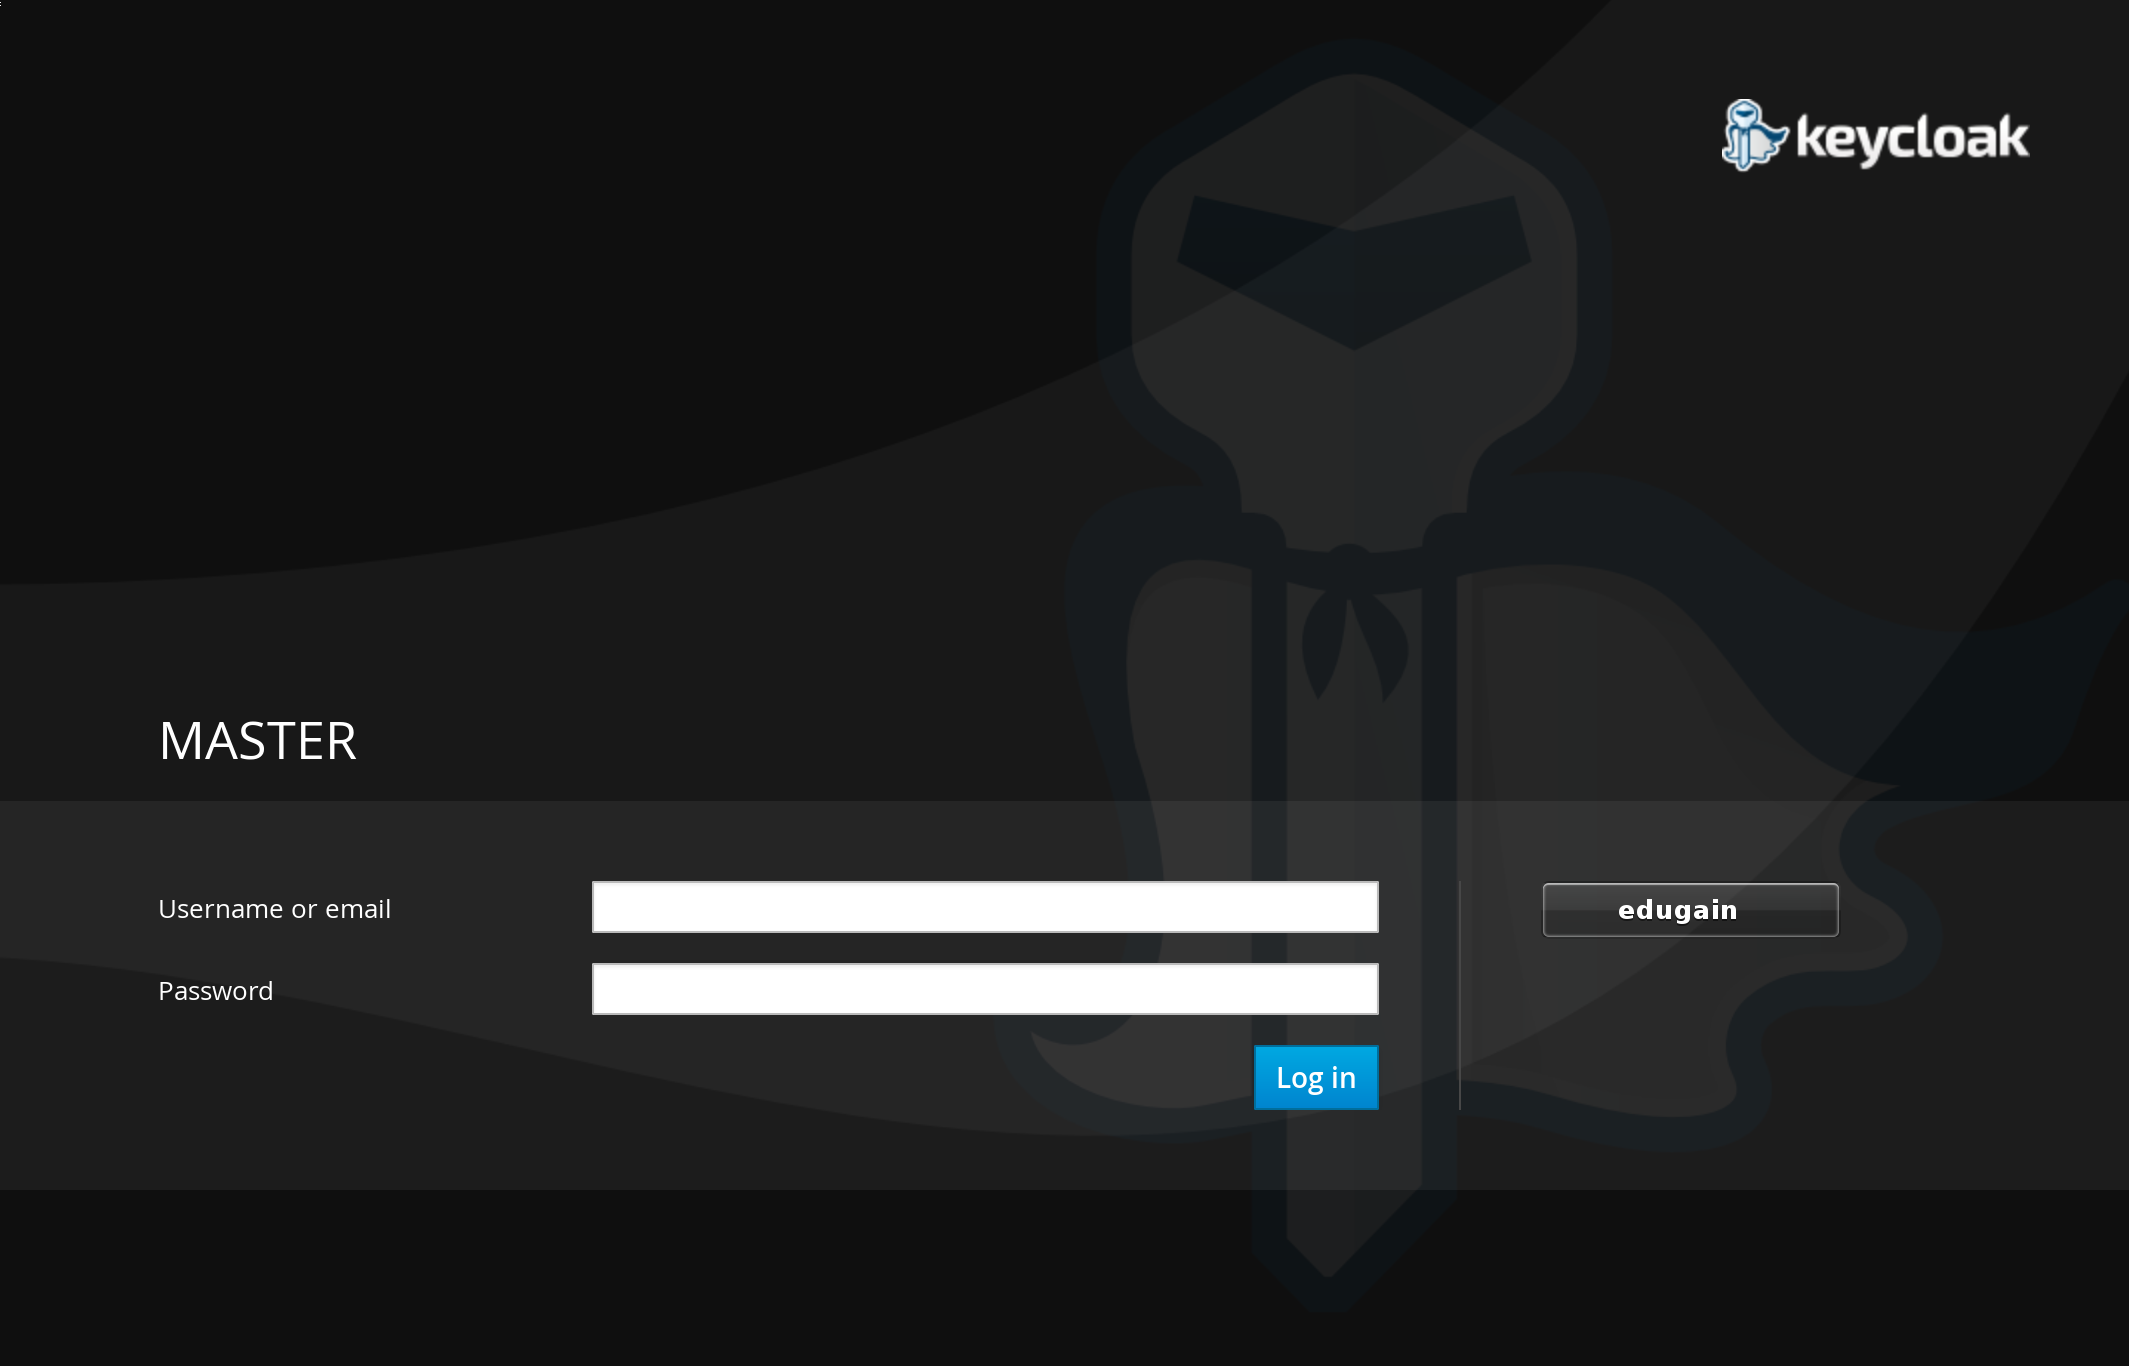
\includegraphics[width=\textwidth]{cyclone-federation-provider-login}\\
    \captionof{figure}{Login screen to CYCLONE Federation Provider.}
    \label{fig:federation-provider-login}
\end{center}

\subsection{Deployment}

The SNET department wish to have an easy way to deploy our software. So we looked into the recommended Docker\footnote{\url{https://www.docker.com/}} application. Docker is an open source application which automates deployment of software applications in linux containers. One of the biggest advantages of the linux containers in Docker is that you have an isolated linux container for each application. Another positive effect of Docker is the Dockerfile. This allows us to define how the software should be deployed and also the dependencies in the application. Our software depends on the mongoDB database so we also liked to have the mongoDB as a own linux container, because we were not sure where the database run in a produktiv environment. Docker give us the ability to define a sequence of how to start the created containers, because the database have to run befor our applications starts. For this we needed a docker-compose.yml file which defines all necessary settings for the containers to start.

\vspace{0.5cm}

\section{iOS}

\begin{description}
\item[System Requirements:] \hfill \\
\begin{itemize}
  \item \textbf{Operating System:} Version: iOS9; Build:13A340
  \item \textbf{Screen Size} 640 x 1136 pixels (~326 ppi pixel density); 4 inches
  \item \textbf{Bluetooth:} v4.0, A2DP, LE
  \item \textbf{Internet Technology:} Wi-Fi
\end{itemize}
\end{description}

The iOS application provides the user with a map of the specific hotspot. For this project the example of indoor navigation inside the Mensa has been implemented. The app shows two floors of the Mensa, together with additional information about the location.

\subsection{Floor plans}
In order to show positions of the user and friends with the exact coordinates on the map, the floor plan material is added as MKOverlay on top of the MKMapView provided by Apple. We use the PDF files provided by \textit{Studentenwerk Berlin} for this project.

Apple also provides registered iOS developers with a framework to manage the mapping of x/y coordinates of the PDF file with the exact Latitude/Longitude real world coordinates of the map
\textbf{(see Figure:~\ref{fig:map1})}.

This framework has been used for this project to integrate the floor plan of the Mensa \cite{AppleFootprint}. The GeoAnchor class provided by Apple converts each corner of a PDF rectangle into a MKMapPoint. The collection of MKMapPoints is combined to a MKPolygon which is used to draw elements and annotations on top of a map. This technology is used to divide the floor plan material into multiple map-tiles that can be added to the map \textbf{(see Figure:~\ref{fig:map2})}.


\begin{figure}
\centering
\begin{minipage}{.5\textwidth}
  \centering
  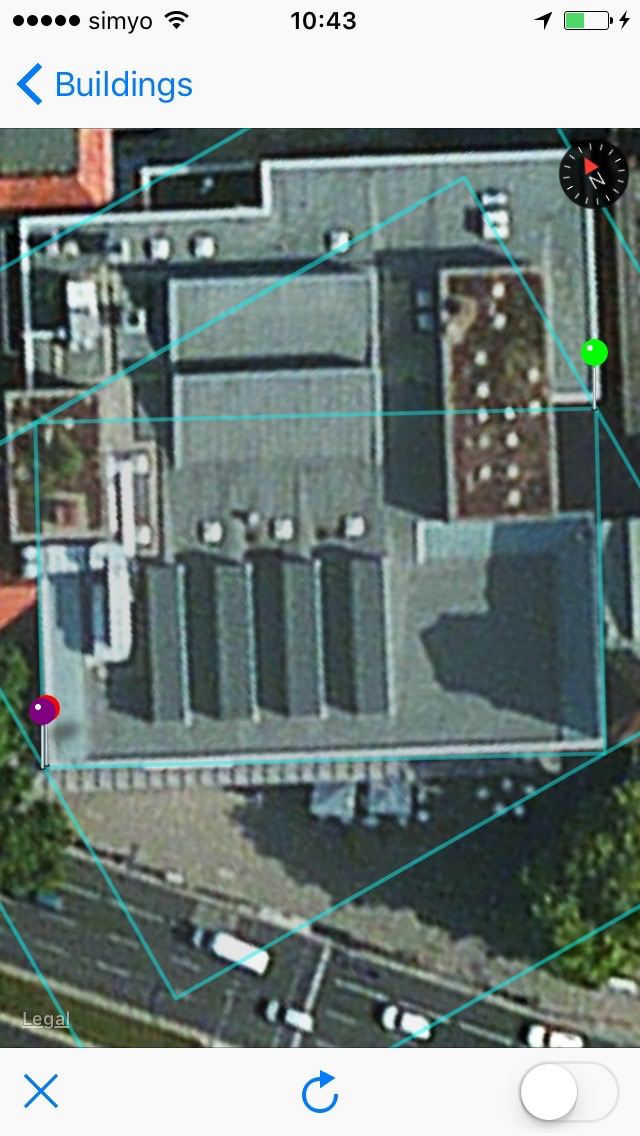
\includegraphics[width=.5\linewidth]{map1}
  \captionof{figure}{Defined Anchor Points and Boundaries}
  \label{fig:map1}
\end{minipage}%
\begin{minipage}{.5\textwidth}
  \centering
  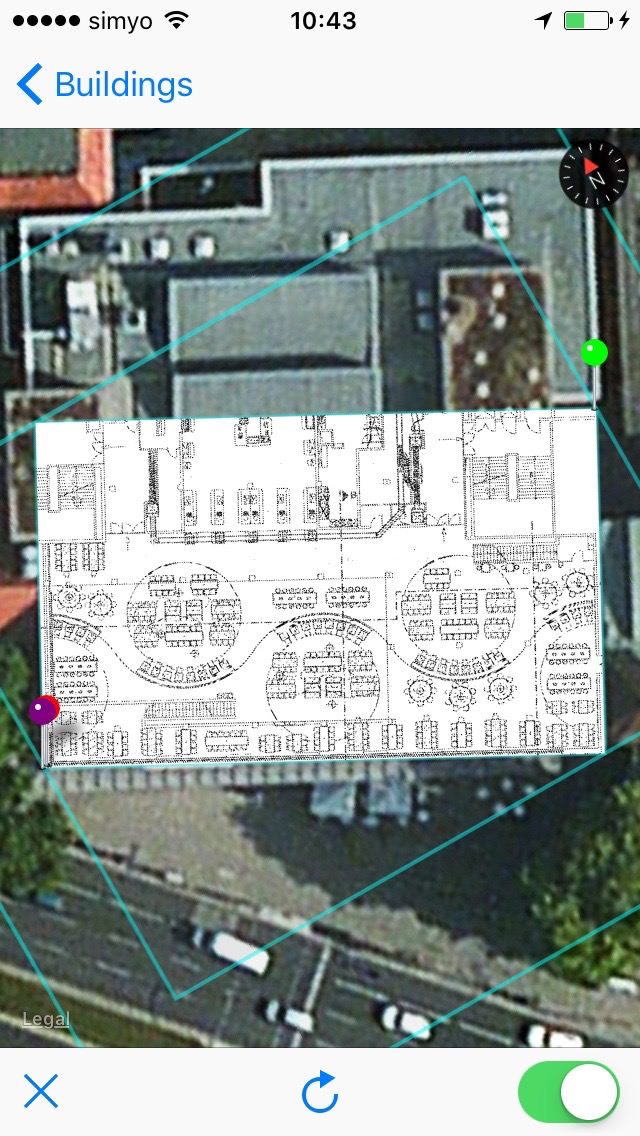
\includegraphics[width=.5\linewidth]{map2}
  \captionof{figure}{Applied Floor plan to the defined Boundaries}
  \label{fig:map2}
\end{minipage}
\end{figure}


\subsection{Login}

In order to use the application, the user has to login via Federation Provider, to get
a security token which grants access to the application server. \\

The app handles the login process using a UIWebView. The login request will then be redirected
to the tubIT login page \textbf{(see Figure:~\ref{fig:login1})}, in which the user finally can type in tubIT username and password.
If the user credentials are correct, the web-view gets redirected to the piazza application server.

If the web-view was able to access the application server successfully, the web-view closes and grants the user access to the application. The web-view can not be bypassed without a successful login via Federation Provider \textbf{(see Figure:~\ref{fig:login2})}. Each request to the application server re-opens the web-view again, if the used security token is invalid or if the user has been logged out.


\begin{figure}
\centering
\begin{minipage}{.5\textwidth}
  \centering
  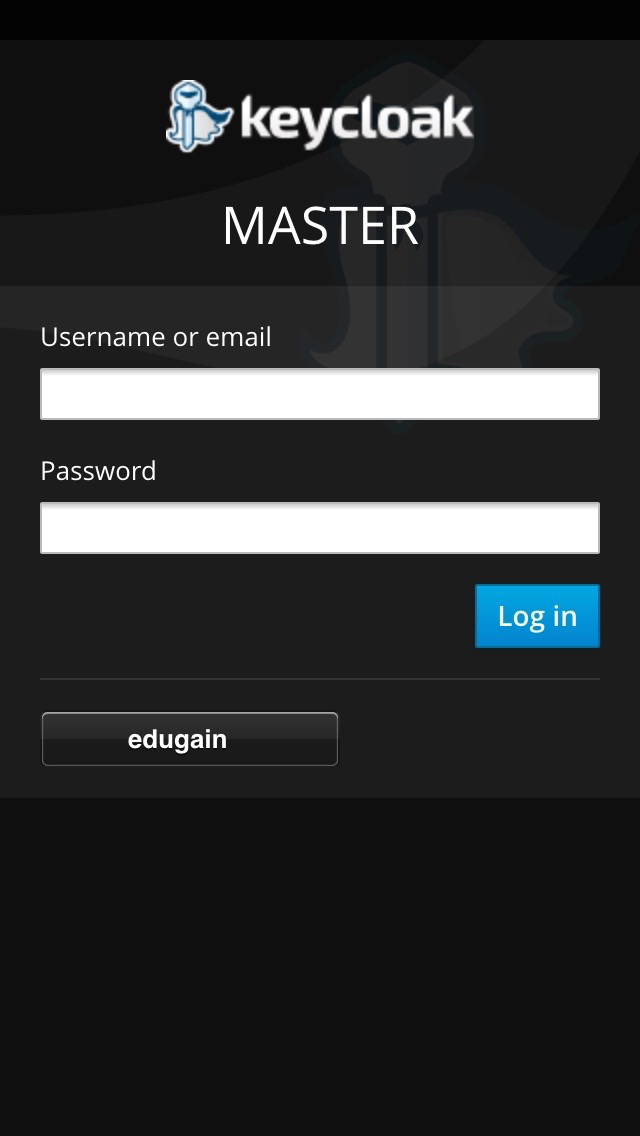
\includegraphics[width=.5\linewidth]{login1}
  \captionof{figure}{Keycloak/Federation Provider}
  \label{fig:login1}
\end{minipage}%
\begin{minipage}{.5\textwidth}
  \centering
  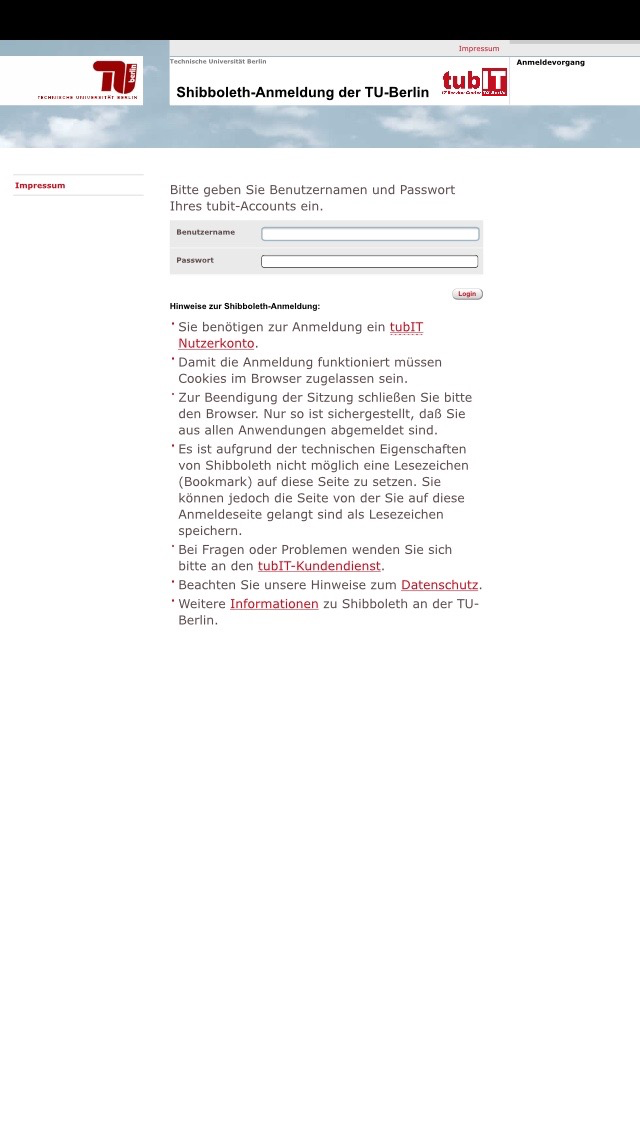
\includegraphics[width=.5\linewidth]{login2}
  \captionof{figure}{Tubit Login Page}
  \label{fig:login2}
\end{minipage}
\end{figure}

\subsection{Hotspots/ Buildings}

\begin{figure}
\centering
\begin{minipage}{.5\textwidth}
  \centering
  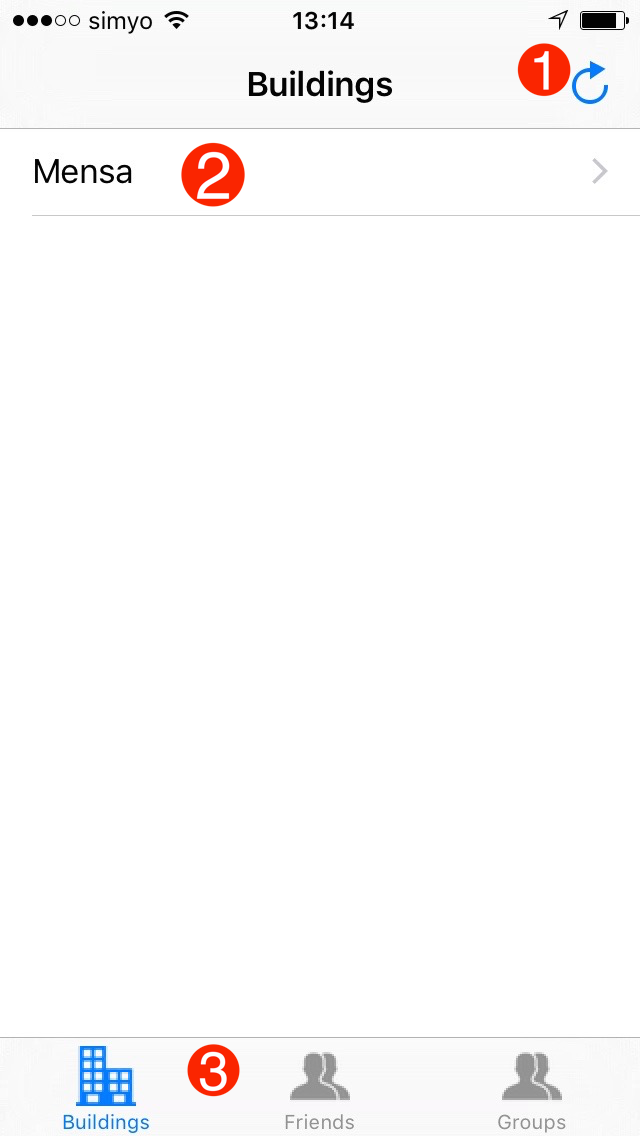
\includegraphics[width=.5\linewidth]{showbuildings}
  \captionof{figure}{List of available Hotspots}
  \label{fig:showbuildings}
\end{minipage}%
\begin{minipage}{.5\textwidth}
  \centering
  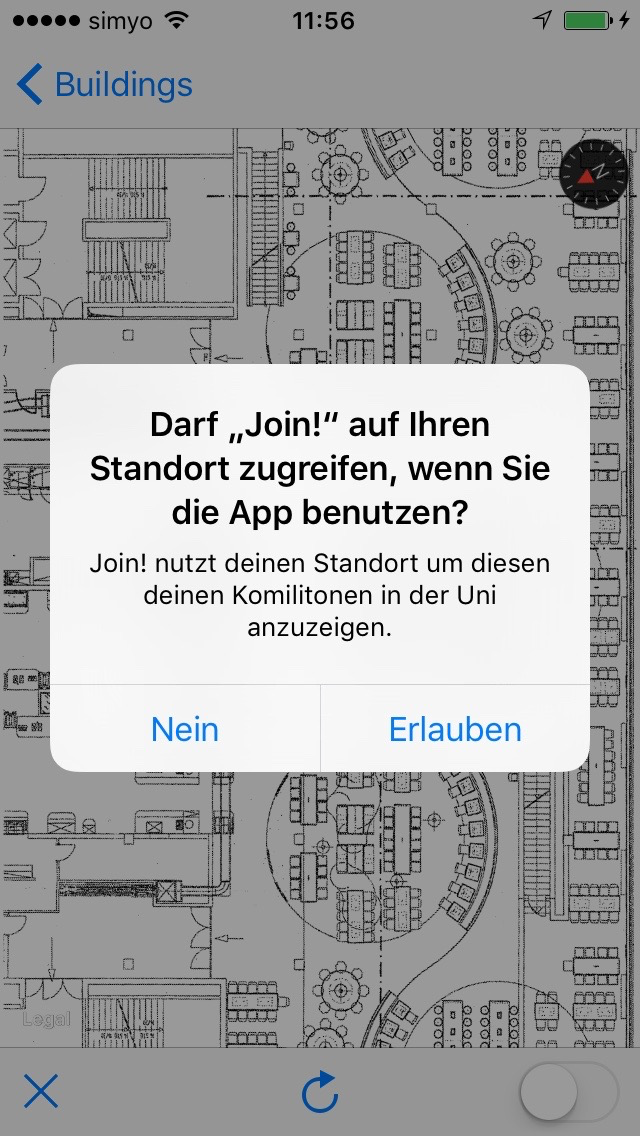
\includegraphics[width=.5\linewidth]{request1}
  \captionof{figure}{Access Location Request}
  \label{fig:request1}
\end{minipage}
\end{figure}



The Buildings View \textbf{(see Figure:~\ref{fig:showbuildings})} is the first view the user sees after login. This view enlists all available hotspots delivered by the backend.

\begin{enumerate}
  \item The reload button, calls the backend to get a list of available hotspots. The list contains the hotspots and the available beacon and floor information.
  \item The Table-view lists all available hotspots from the backend. Each cell contains the name of a Hotspot.
  \item The Application is divided into three contextual distinct parts: Buildings, Friends and Groups. This subdivision is implemented in a UITabBar which is the leading element of the application architecture.
\end{enumerate}

\subsection{Indoor Positioning}

\begin{figure}
\centering
\begin{minipage}{.5\textwidth}
  \centering
  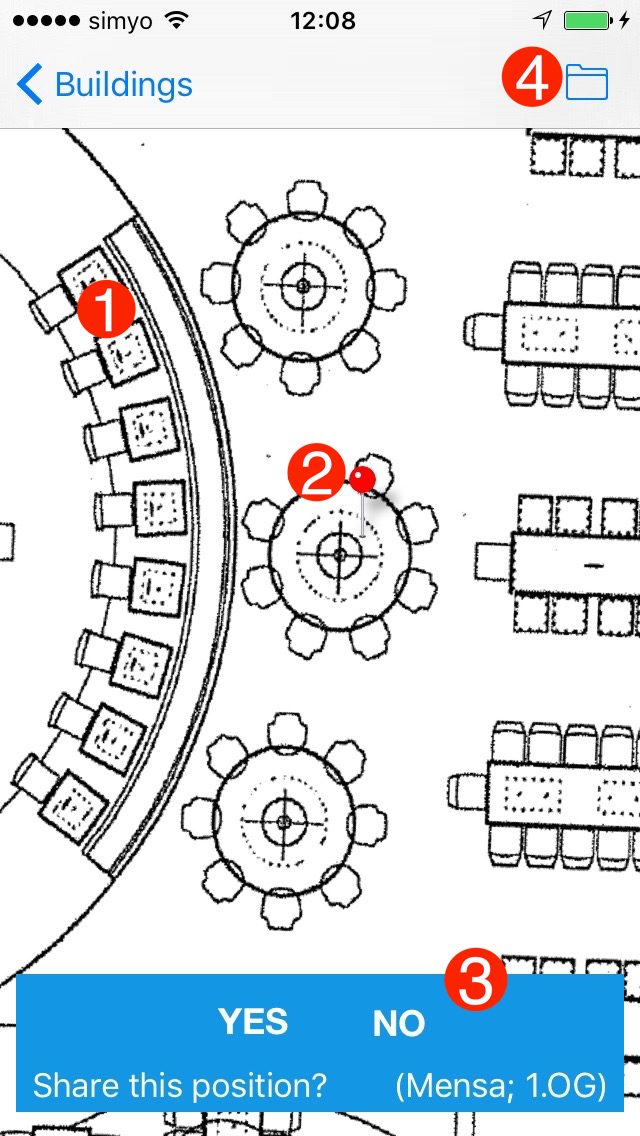
\includegraphics[width=.5\linewidth]{shareposition}
  \captionof{figure}{Share Position Mode}
  \label{fig:shareposition}
\end{minipage}%
\begin{minipage}{.5\textwidth}
  \centering
  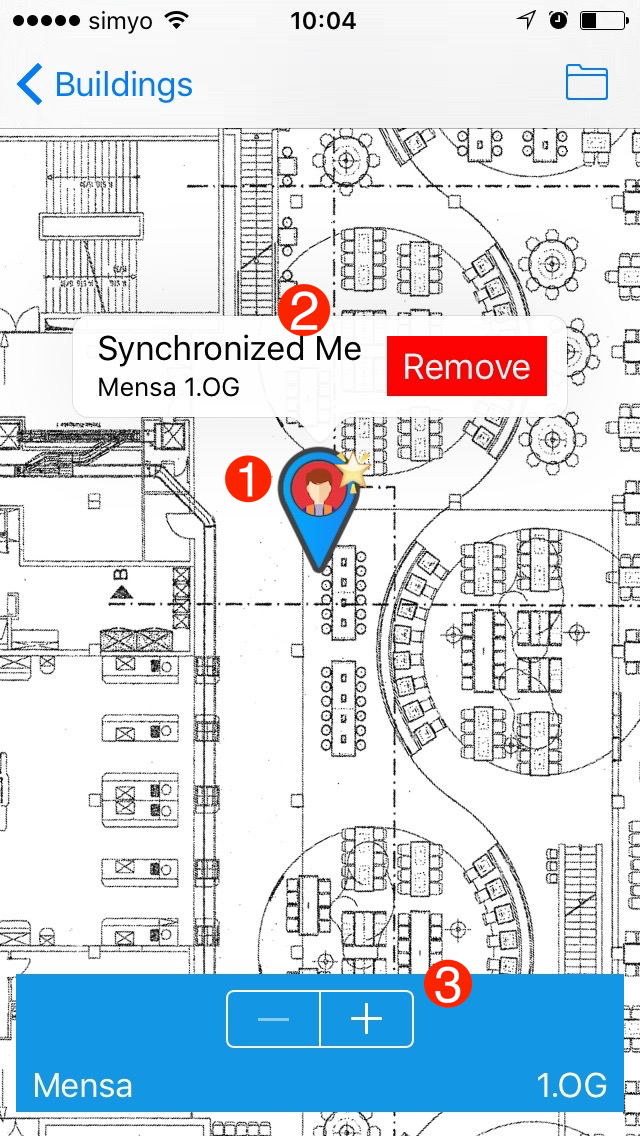
\includegraphics[width=.5\linewidth]{synchronizedme}
  \captionof{figure}{Synchronized Position Mode}
  \label{fig:synchronizedme}
\end{minipage}
\end{figure}


If the user taps on one of the buildings enlisted, the app opens respectively
the corresponding floor plan in an MKMapView \textbf{(see Figure:~\ref{fig:shareposition})} that shows the mensa floor plan on a large scale. This improved scale functionality was added additionally in order to increase the usability and accuracy of manual pin-pointing.

\begin{enumerate}
\item The the Map-view shows the first floor of the Mensa by default, if the Tubit-MSE api which provides the floor and building information is not available. In cases of availability of the Cisco-MSE api, the Map-view shows the corresponding floor as soon as the Map-view appears on the screen.

\item The manual pin pointing of the users position is triggered by a so called long press on the map which was additionally implemented. The long press is a distinct user-interaction mode. It is applied as solution for manual pin pointing on iOS in order to prevent the user from mistakenly share  positions by inadvertently touching the map. After a long press is registered by the system, it drops a red pin on the position where the user pressed. This switches the Map-view into a share position mode. In this mode the user can touch on any place on the map to easily edit or remove the pin, if the position to share is not correct.

\item The information panel is used to give the user the possibility to change the floor by pressing the plus (up) or minus(down) button. The Information-Panel also flips with an animation, signaling the user of the changed mode of the MapView. The flip animation is triggered as soon as the system successfully registers a long press. In Share Position Mode the Information-Panel prompts the user to share the location.

\item The File-Button modally opens a settings view with further options.
\end{enumerate}


\textbf{Figure:~\ref{fig:synchronizedme}} shows the MapView after a user has successfully shared the position either via Bluetooth Beacon, automatically using the Apple CLLocation Framework or manually via pin-pointing.


\begin{enumerate}
\item As soon as the backend has received the new location of the user successfully, the red pin is exchanged with a marker-annotation. This marker shows the provided synchronized location of the user. The switch of the marker gives the user a hint, that his position is now synchronized with the server state. This marker is also used for the positions of friends, however the user position is highlighted with a star.
\item If the user taps on his own marker, it reveals an annotation-view that includes the user name as well as a remove button that deletes the shared position from the server permanently (In this project the username "Synchronized Me" was used for debugging).

\item The Information-Panel is now flipped back to Normal mode or to Synchronized Position Mode if the user previously shared the position manually.
\end{enumerate}


The Settings view (\textbf{see Figure:~\ref{fig:settings1} and ~\ref{fig:settings2}}) provides additional options to indoor positioning and information markers that are shown on the floor plan.

\begin{figure}
\centering
\begin{minipage}{.5\textwidth}
  \centering
  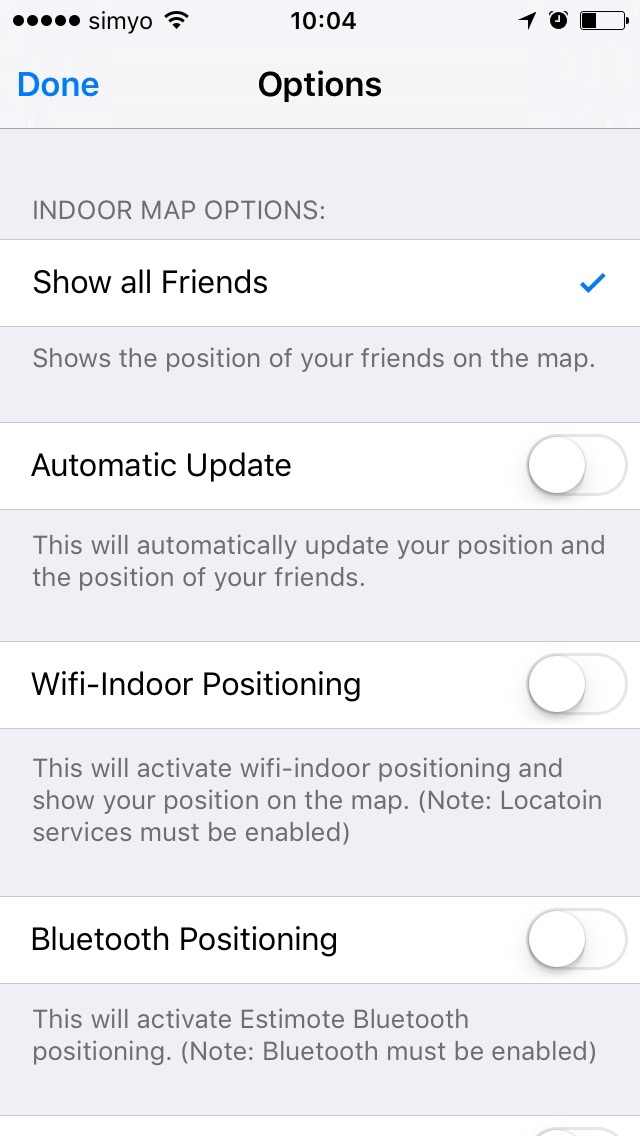
\includegraphics[width=.5\linewidth]{settings1}
  \captionof{figure}{Map Settings 1}
  \label{fig:settings1}
\end{minipage}%
\begin{minipage}{.5\textwidth}
  \centering
  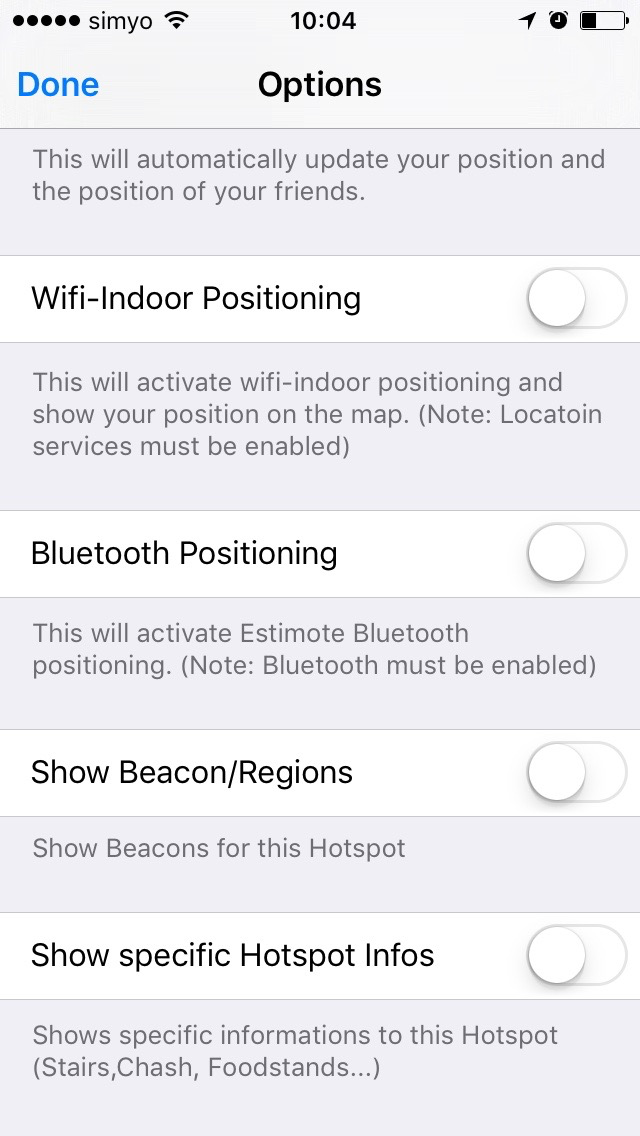
\includegraphics[width=.5\linewidth]{settings2}
  \captionof{figure}{Map Settings 2}
  \label{fig:settings2}
\end{minipage}
\end{figure}

\begin{enumerate}
\item \textbf{Show all Friends} activates markers for friends in the same hotspot. \textbf{(Note: Friends will only be shown on the map if the user has shared his own position before)}
\item \textbf{Automatic Update} activates a routine that constantly requests the server for location updates of friends.
\item \textbf{Wi-Fi Indoor-Positioning} activates the CLLocation Framework positioning. This will automatically update the user position while moving through the building.
\item \textbf{Bluetooth-Positioning} activates location sharing via Bluetooth beacons
\item \textbf{Show Beacons/Regions} activates annotations showing Beacons placed in the hotspot
\item \textbf{Show Specific Hotspot-Information} activates annotations showing specific hotspot informations.
\end{enumerate}

If the user activates \textbf{Show all Friends} on settings and has already shared the own position, the map-view adds markers for each friend located in the same hotspot. The friend markers are equipped with Accuracy-Circles placed underneath the marker. The radius of the Accuracy-Circles decreases with the accuracy of the shared position. If a position is manually shared, no Accuracy-Circle will be shown. However, if the position is shared via Bluetooth or WiFi, the Accuracy-Circle increases to show the region the friends position \textbf{(see Figure:~\ref{fig:showfriends})}.

If the user activates \textbf{Show Specific Hotspot Informations} on settings, the map-view will show the user specific informations regarding the Hotspot such as Cash-register or Foodstands. This functionality has been added in order to improve the usability of the floor plan and helps the user to orientate using the map while navigating in the building \textbf{(see Figure:~\ref{fig:additionalinfo})}.

\begin{figure}
\centering
\begin{minipage}{.5\textwidth}
  \centering
  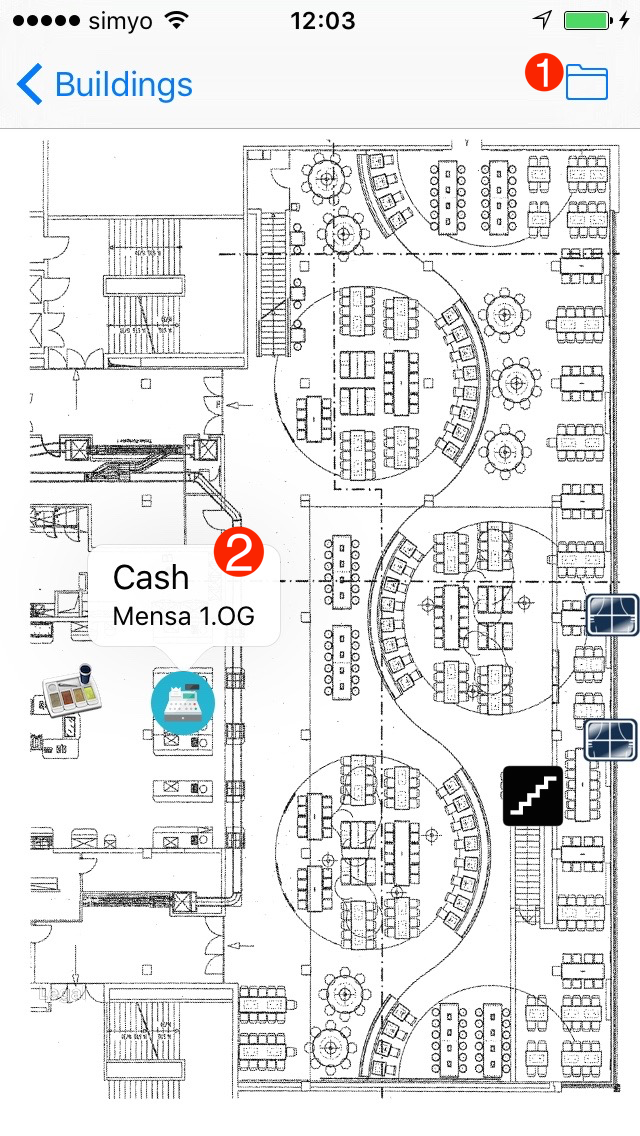
\includegraphics[width=.5\linewidth]{additionalinfo}
  \captionof{figure}{Additional Hotspot Informations}
  \label{fig:additionalinfo}
\end{minipage}%
\begin{minipage}{.5\textwidth}
  \centering
  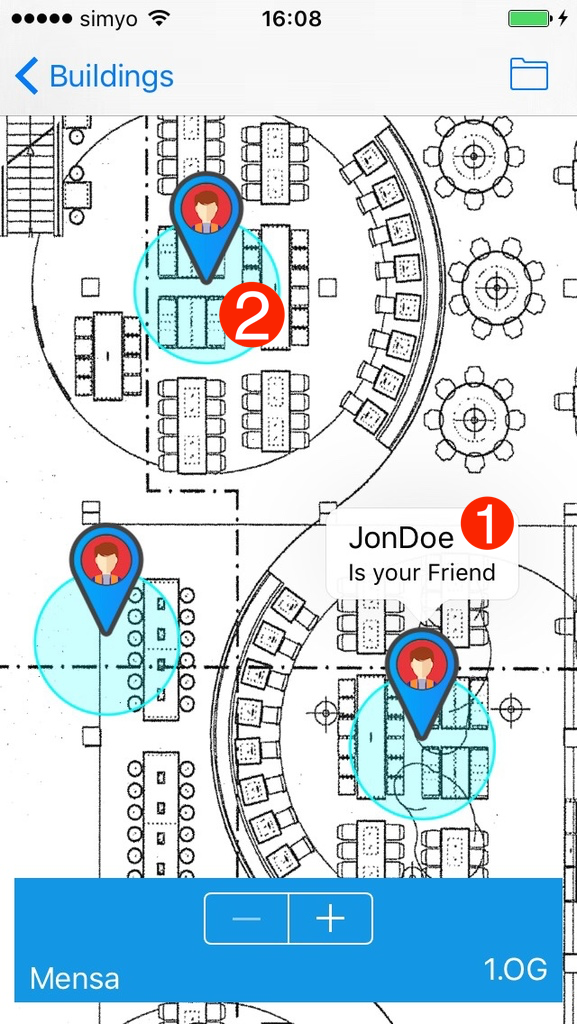
\includegraphics[width=.5\linewidth]{showfriends}
  \captionof{figure}{Friends in this Hotspot with Accuracy}
  \label{fig:showfriends}
\end{minipage}
\end{figure}


\subsection{Friends}

As soon as the user taps on the All Friends button of the TabBar, the application shows the All my Friends List \textbf{(see Figure:~\ref{fig:friendlist})}. This view shows either the friends of the user or opens companion requests that the user needs to accept in order to add a person into his friends-list. Note that all available friends will be shown in this list regardless of their group affiliation.

\begin{figure}
\centering
\begin{minipage}{.5\textwidth}
  \centering
  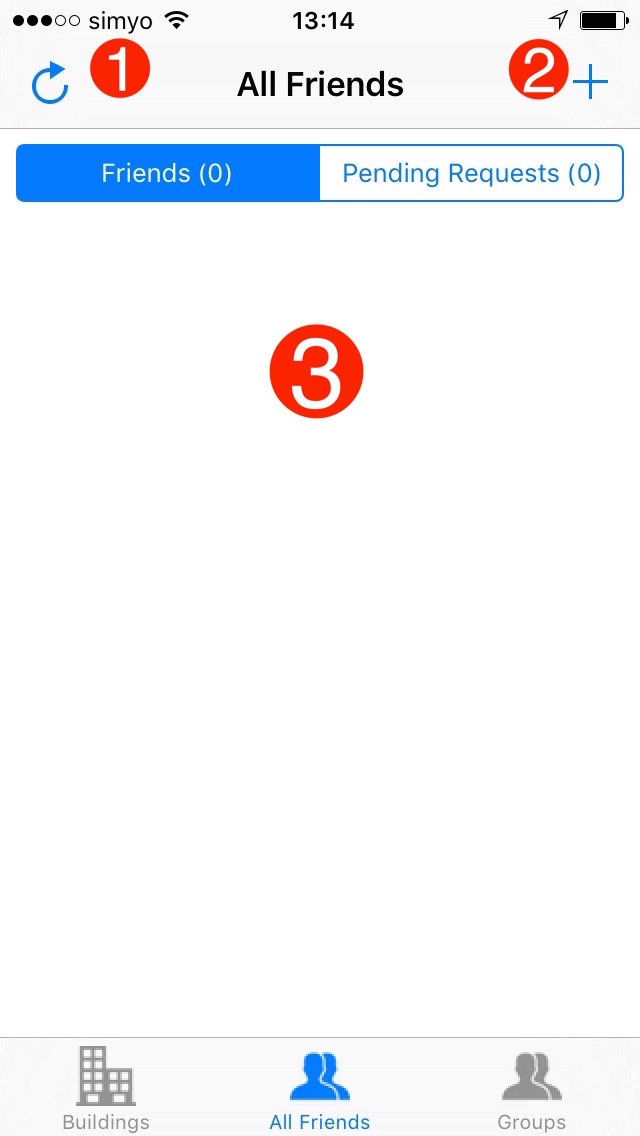
\includegraphics[width=.5\linewidth]{friendlist}
  \captionof{figure}{Available Friends and Open Requests}
  \label{fig:friendlist}
\end{minipage}%
\begin{minipage}{.5\textwidth}
  \centering
  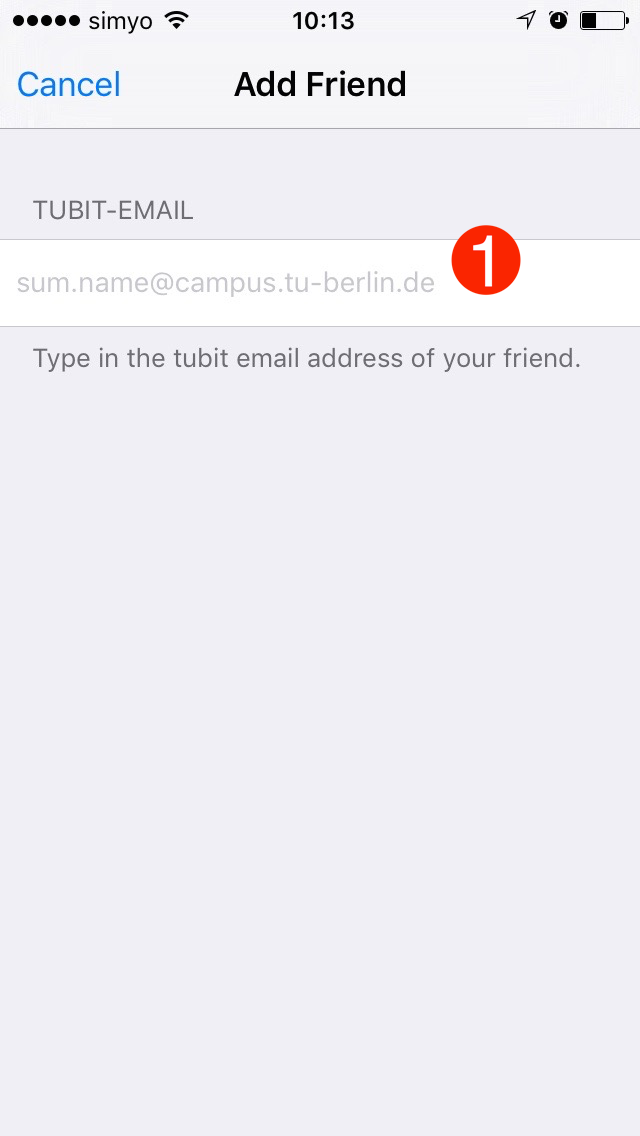
\includegraphics[width=.5\linewidth]{addfriend}
  \captionof{figure}{Add Friends}
  \label{fig:addfriend}
\end{minipage}
\end{figure}

\begin{enumerate}
\item The Reload-button is implemented in order to update the list of friends or new companion requests. In future work the server should be able to send remote notifications in order to inform the user of new companion requests.

\item The Plus button is implemented to open a new view \textbf{(see Figure:~\ref{fig:addfriend})} where the user can add new friends and send new companion requests.

\item The list-view is managed by a UISegmentControl. The content is divided into available friends and available companion requests which are shown by numbers. A tap on one of the segments will either change the content of the Table-view to friends or companion requests. The entry of the list contains the provided name of a friend.
\end{enumerate}


As seen on \textbf{(Figure:~\ref{fig:addfriend})}, the app opens modally a new view that enables the user to add new friends.

\begin{enumerate}
\item The UITextfield is used in order to enable the user to type in the email address of a friend. This request will be handed by the backend. The response of the backend about the success or fail of the request will be directly shown underneath the textfield.
\end{enumerate}

\subsection{Groups}

\begin{figure}
\centering
\begin{minipage}{.5\textwidth}
  \centering
  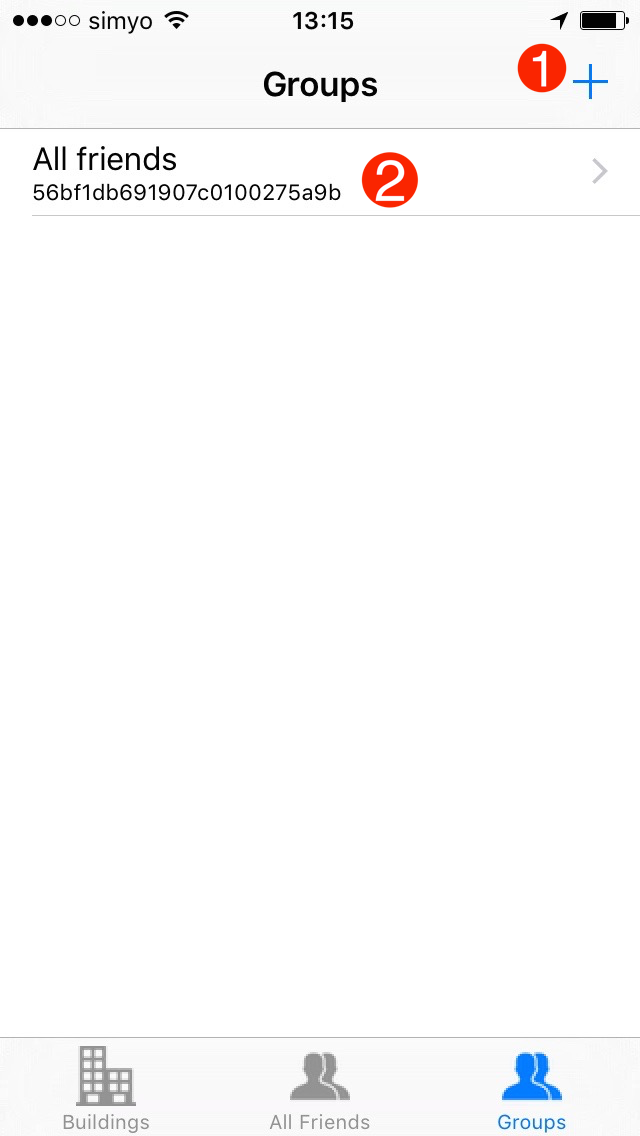
\includegraphics[width=.5\linewidth]{showgroups}
  \captionof{figure}{Show available groups}
  \label{fig:showgroups}
\end{minipage}%
\begin{minipage}{.5\textwidth}
  \centering
  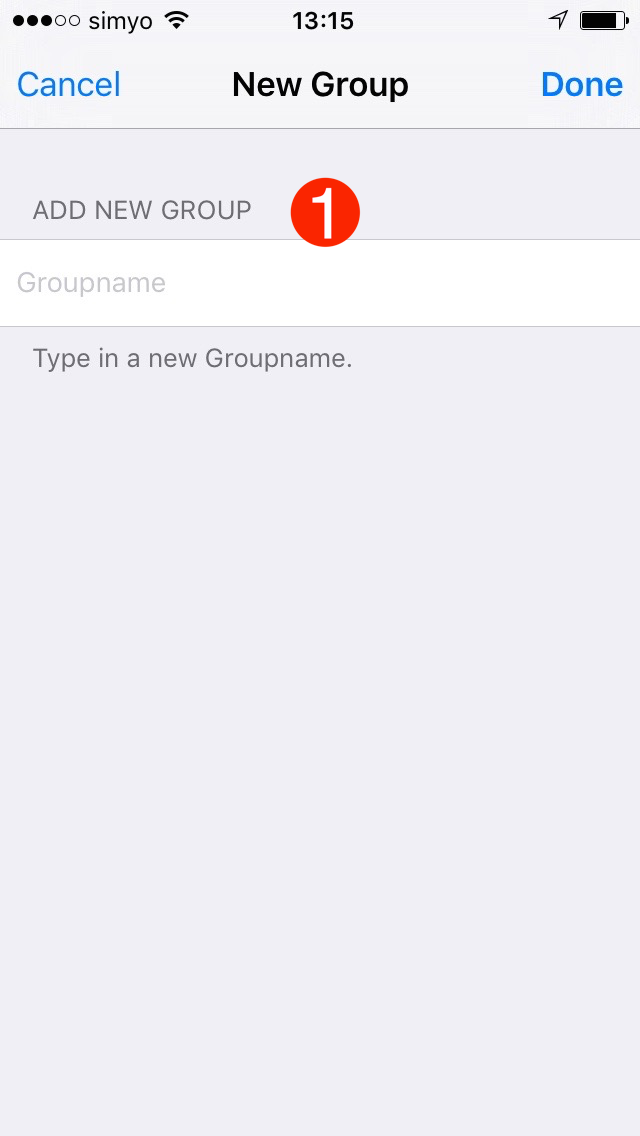
\includegraphics[width=.5\linewidth]{addgroup}
  \captionof{figure}{Add new group}
  \label{fig:addgroup}
\end{minipage}
\end{figure}

The backend enables the user to manage groups. Each user has a group named All friends, containing all of the users friends. Additionally the user may have different friends that can be added to own groups. These groups will be enlisted in this Table View as shown in \textbf{(see Figure:~\ref{fig:showgroups})}.

\begin{enumerate}
 \item The plus-button will open a new view modally that enables the user to create a new group (\textbf{(see Figure:~\ref{fig:addgroup}}).
 \item This tableview shows all available groups of the user. Each cell contains of the Name of the group together with the GroupID as subtitle. For future work if the user taps a group, it will open a new list showing the members of this group. The user should also be able to add specific friends to a group as well as edit or delete a group.
\end{enumerate}

\subsection{Geofencing}
The iOS client supports Geofencing abilities for registered Hotspots. Geofencing notifies the app when its device enters or leaves the geographical region of a hotspot. For this project the triggered notification greats the user and acts as a reminder to use the app if the user enters the Mensa. The notification can also be used to take the user in charge of the decision whether he wants to download updates about the hotspot. The notification will also act as a reminder to deactivate Bluetooth if the user leaves the Mensa to save battery.


\subsection{Future Work on iOS}
The iOS client build for the project shows a proper solution of mobile indoor navigation backed with a scalable backend system. However some functionalities may be added to the client as they have been out of scope to this project.

\begin{description}
  \item[Remote Notifications] \hfill \\
  Remote notification handling is state of the art in mobile applications of these days. It should be considered to equip the backend with the ability to notify a user if one of his friends shared his position in a specific hotspot, instead of constantly polling for updates. Remote Notifications would also be used to notify the user for new companion requests. Also scheduled polling for hotspot updates is not a best practice and should be exchanged by a publish-subscribe pattern.
  \item[CLLocation Framework] \hfill \\
  In future work, the new CLLocation framework should be considered as first choice technology for indoor navigation on iOS devices. Authorities of locations that are interested in indoor navigation on iOS should consider an enrollment on Apples Map Connect program \cite{MapsConnect}. With a successfull enrollment, floor information as well as the accuracy of the users position would be improved.
  \item[Friends/Group Management] \hfill \\
  In future work, the client should give the user more posibilities to manage his friends as moving friends to specific groups or edit groups. The map should also be equipped with the posibilities to show specific groups instead of only all friends in a hotspot.

\end{description}

\vspace{0.5cm}

\section{Android}

Android application enables user to manage companions, automatically and manually retrieve users indoor position using different localization techniques available, share position with friends and show friend's positions on indoor maps. Application currently includes indoor maps of the Mensa in Hardenbergstraße at TU Berlin.

Application requires Android version 5.0 or higher. It uses API level 21. Application was tested on Nexus 4 and Nexus 5 devices.

\subsection{Floor plans}
Application show floor plans as overlays over Google Maps. We use floor plans in the PDF format provided by \textit{Studentenwerk Berlin} for purpose of this project. PDF files were converted to PNG files and shown on top of Google Maps using \textit{GroundOverlay} class. Different floors are represented with multiple floor plans.

\subsection{Login}
To authenticate with backend server, application has to send authentication token with every requests it sends. Application retrieves authentication token during login procedure. Login is done with Federation Provider project. During login procedure, user is shown login page in web view inside the mobile application. After successful login application stores the retrieved authentication token in \textit{shared preferences} and user it for future requests.

\subsection{Communication with backend server}
Application communicates with backend server using REST requests. For performing REST requests application uses \textit{Volley} library.

\subsection{Menu view}
Menu view is the main screen of application as shown in figure \ref{fig:android_menu_view}. It enables user to open a map of a hotspot (1), show groups (2), add companions (3) and manage companion requests (4). User can add friends using email address as shown in figure \ref{fig:android_add_friend}.

\begin{figure}
\centering
\begin{minipage}{.5\textwidth}
  \centering
  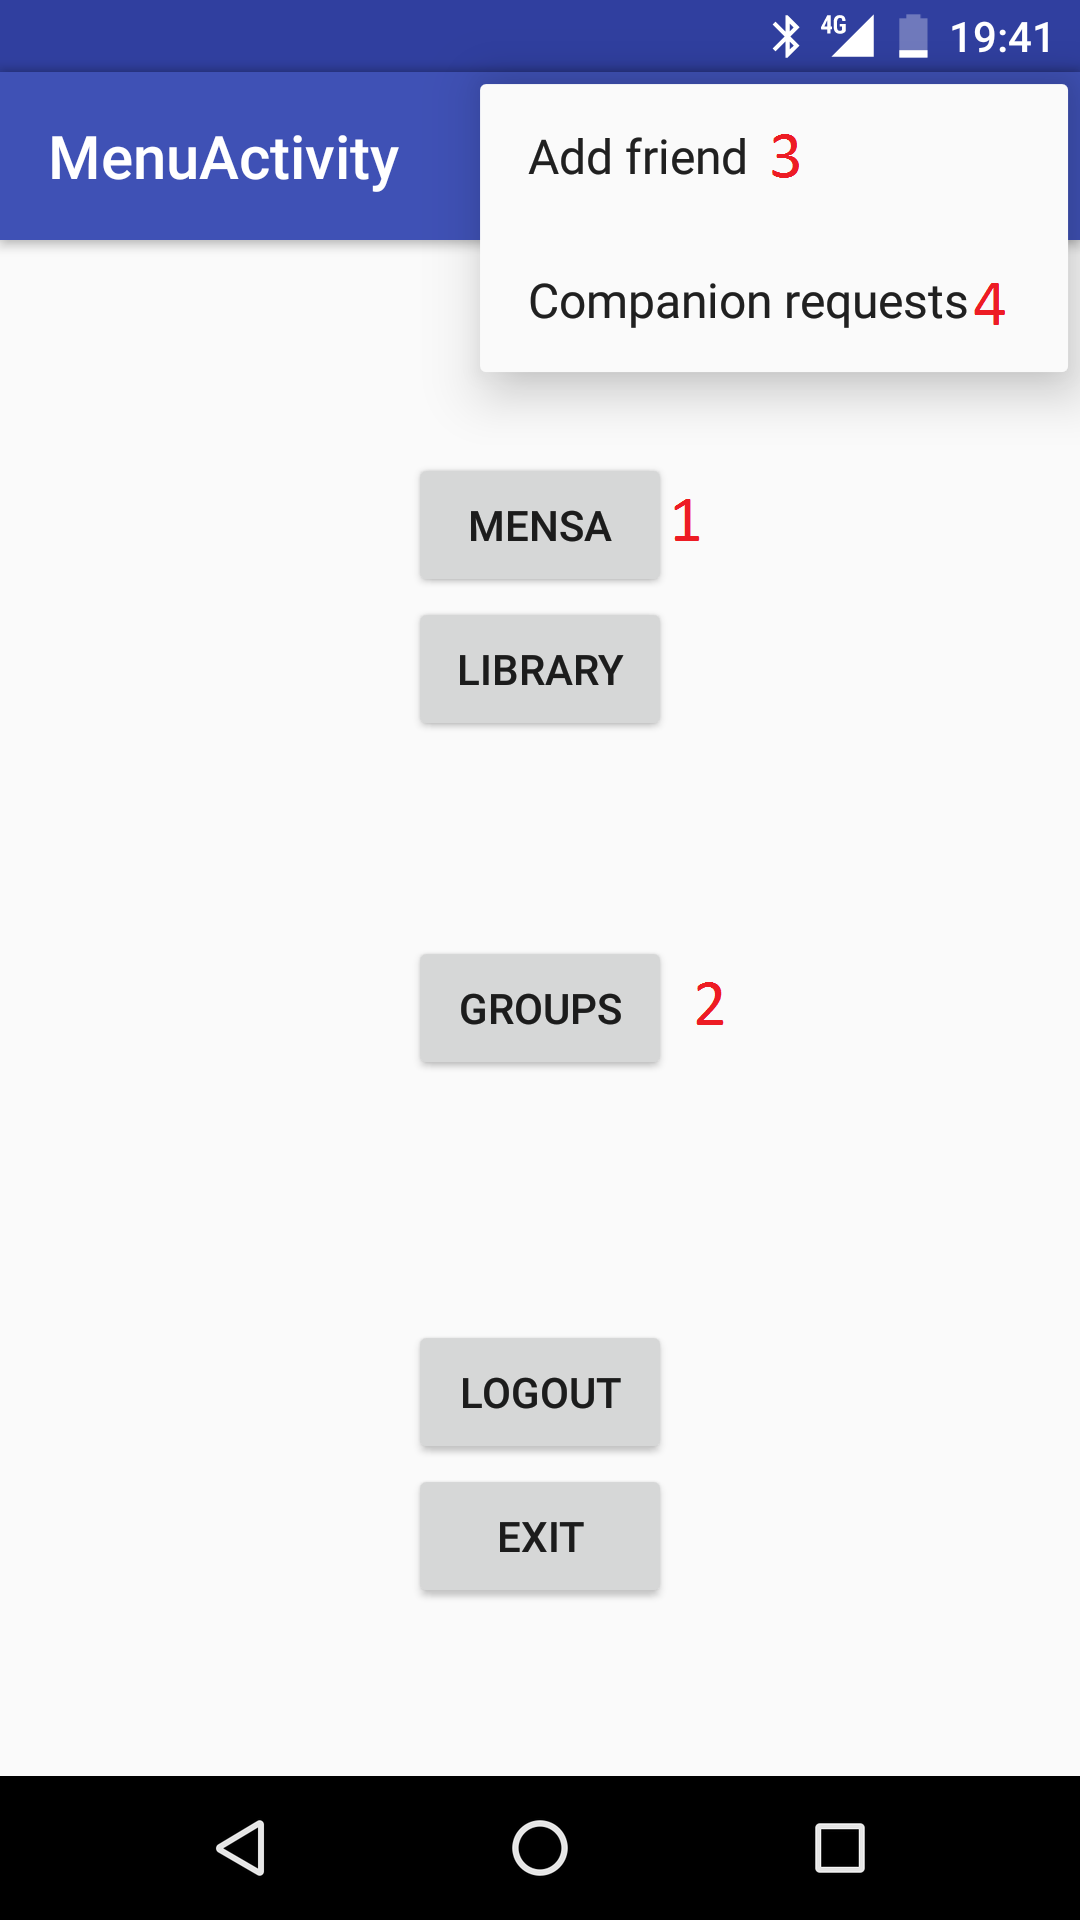
\includegraphics[width=.5\linewidth]{android_menu_view}
  \captionof{figure}{Menu friend}
  \label{fig:android_menu_view}
\end{minipage}%
\begin{minipage}{.5\textwidth}
  \centering
  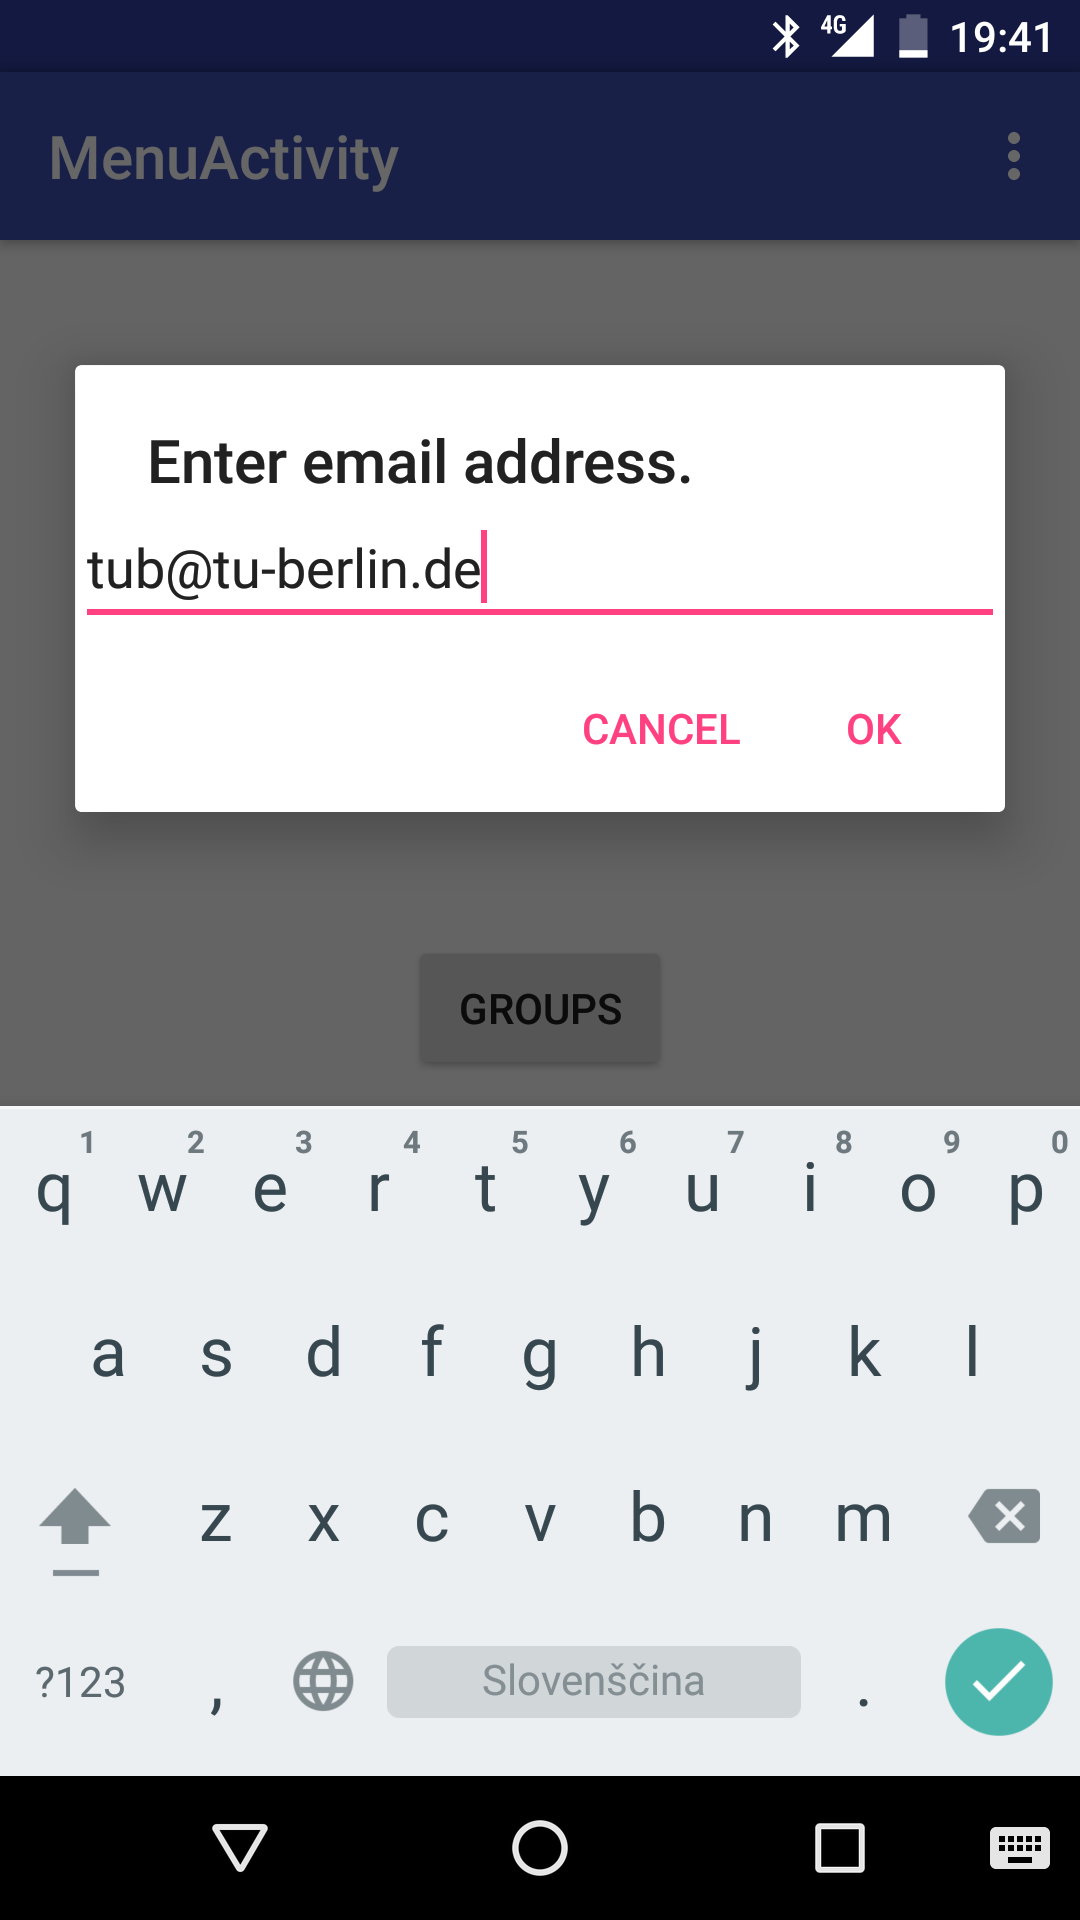
\includegraphics[width=.5\linewidth]{android_add_friend}
  \captionof{figure}{Add friend}
  \label{fig:android_add_friend}
\end{minipage}
\end{figure}

\subsection{Retrieving user's position}
\subsubsection{Cisco MSI API}
Retrieving position from Cisco MSI API provided by tubIT is implemented as a background service. If mobile device has WiFi enabled and it is connected to \textit{eduroam}, service scans the API in 30 seconds intervals. API response is processed and building name and floor information are stored in \textit{LocationSharingSingleton} instance.

\subsubsection{Estimote Beacons}
Searching for nearby Estimote Beacons and Nearables is done using ranging method and nearable discovery method provided by Estimote SDK. All detected Beacons and Nearables are represented as internal \textit{Beacon}. Closest beacon is determined as the one with the best signal strength (RSSI). Information about detected beacons is then stored in \textit{LocationSharingSingleton} instance.

\subsubsection{Manual position pinning}
User can manually pinpoint position on the indoor map of selected hotspost. With checkbox \textit{Share position} (1) user enable manual pinpointing. Position can then be set with marker (2). Manual pinpointing is shown in figure \ref{fig:android_pinpoint}. Pinpointed coordinates and floor are stored in \textit{LocationSharingSingleton} instance.

\begin{figure}
\centering
\begin{minipage}{.5\textwidth}
  \centering
  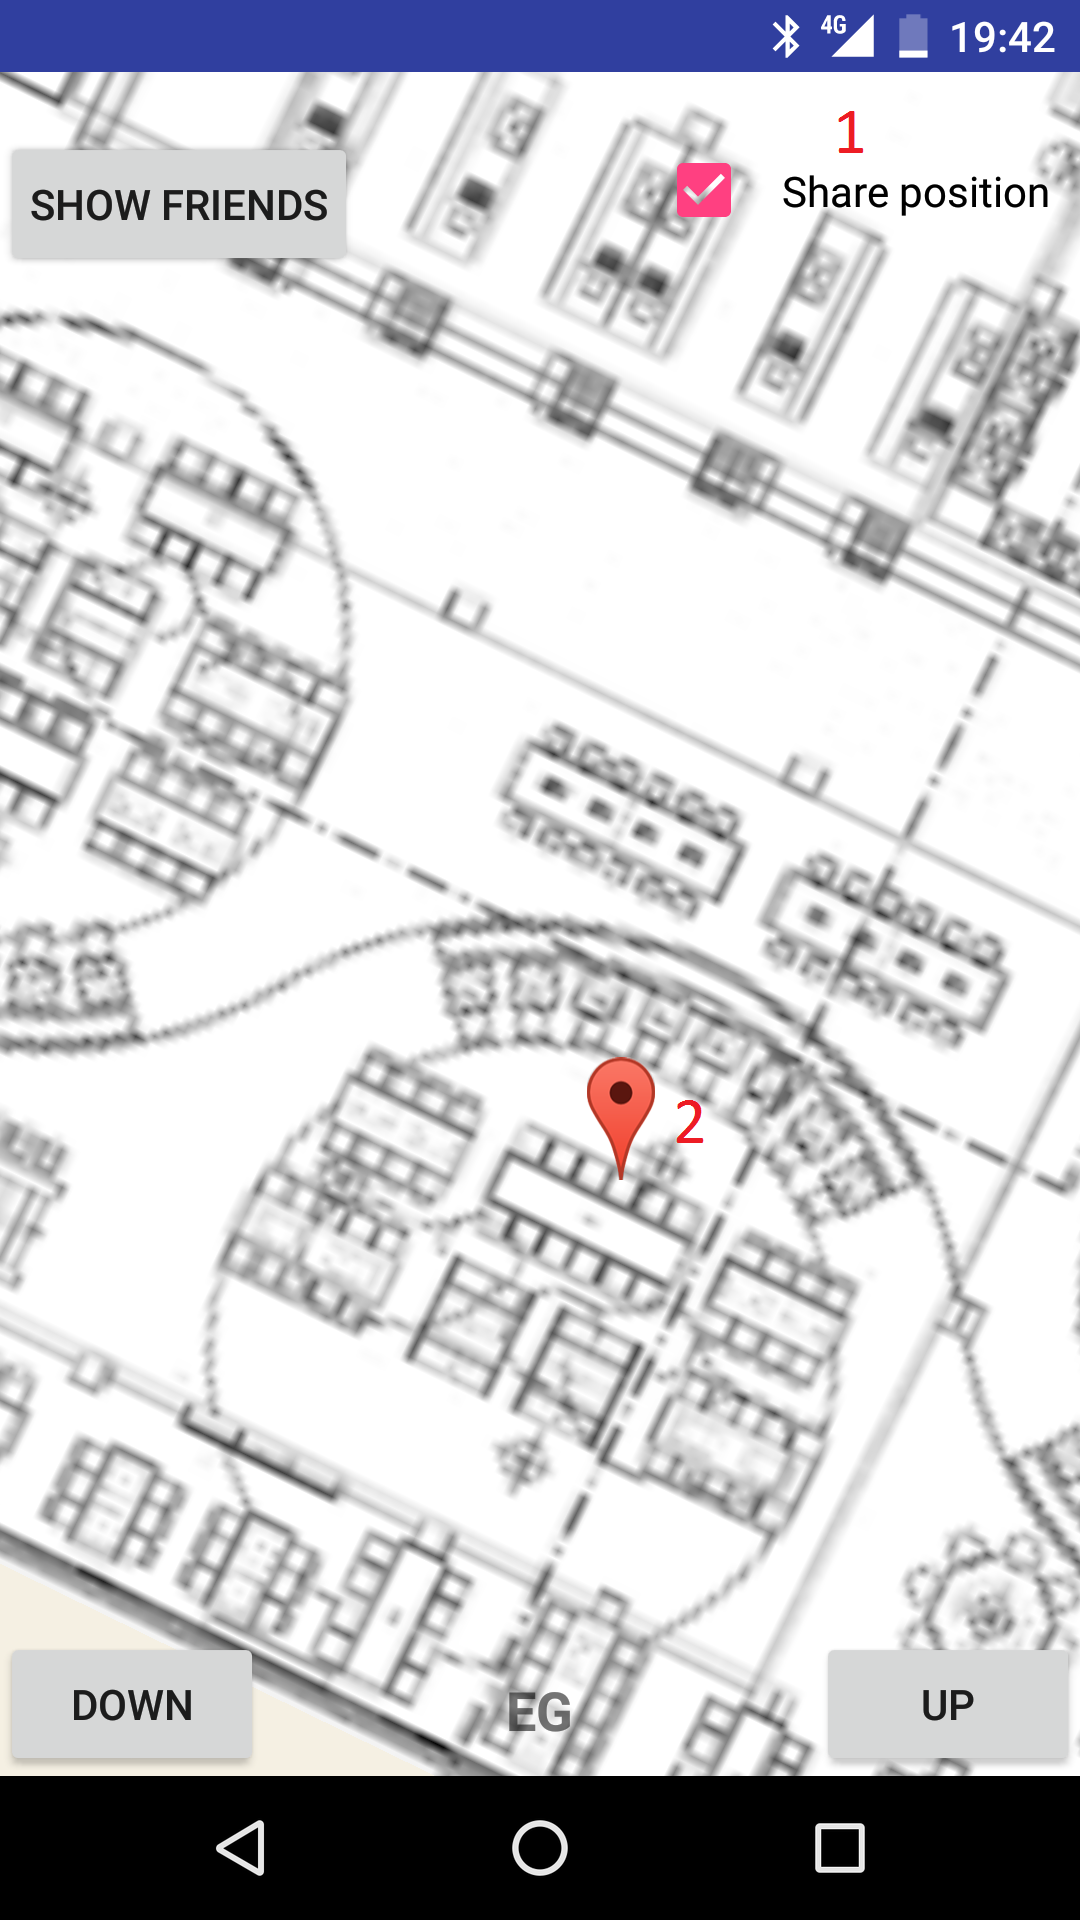
\includegraphics[width=.5\linewidth]{android_pinpoint}
  \captionof{figure}{Manual pinpointing}
  \label{fig:android_pinpoint}
\end{minipage}%
\begin{minipage}{.5\textwidth}
  \centering
  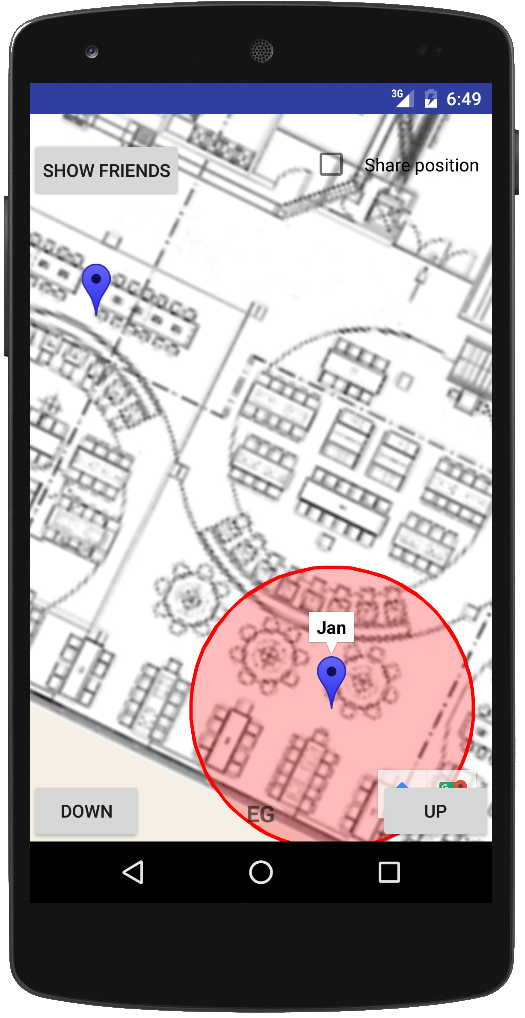
\includegraphics[width=.5\linewidth]{android_show_friends}
  \captionof{figure}{Showing friends}
  \label{fig:android_show_friends}
\end{minipage}
\end{figure}

\subsection{Sharing user's position}
Sharing user's position is implemented with a background service. Every 15 seconds service sends the most accurate location data stored in \textit{LocationSharingSingleton} instance to the backend server. Determining the most accurate position goes as follows; most accurate are manually pinpointed coordinated and floor, followed by beacon identifier that defines a region. The least precise is the MSI retrieved building name and floor information.

\subsection{Showing friends}
Friends in hotspots are shown on the indoor map as shown in figure \ref{fig:android_show_friends}. For different accuracies different markers are used. Pinpointed position is shown with single marker (1). Position shared with beacon ID is shown with marker surrounded by circle representing the region defined by beacon signal strength (2).

\subsection{Future work}
Implemented client application provides basic functionalities for indoor positioning. Proposed future work suggest the functionalities that should be considered in further development of the project.

\begin{description}
  \item[Remote Notifications] \hfill \\
  Backend and could implement sending remote notifications to inform mobile clients about events such as friend entering hotspot.
  \item[Friends/Group Management] \hfill \\
  Current application enables user to list all available groups and friends inside them. Adding and deleting friends is already implemented. Group management is already supported on backend, so mobile application should implement options to add, edit and delete groups and to assign user to one or more groups.

\end{description}
